\section{Main theorem}
\label{sec:main}

\subsection{Setting}
We use the notation of Papers~F, H and~I~\cite{F,H,I} and recall only what the statements need; Sec.~II of~\cite{I} has the full setting.
A periodic window is $p=\mathcal N_V\,\Gamma\,h/Z$ with $h-1=e^{-w^2/2s^2}R(t)$, $R(t)=\sum_{n\ge1}q0_n\cos(nt-\varphi_n)$, $t=k'v$.
We write $x=(k'\sigma)^2$, $\eta=\sup|R|$, $\ell=\ln(1/\sigma)$, $B=b/\sigma^2$ and $\Gamma_\ell=\sqrt{(1+10/\ell)/\ell}$.
A window is \emph{admissible} if it satisfies (P0), (P2)--(P4), (P6) of~\cite{F} and $5\times10^{11}\sigma^2\le x\le0.003$; by (P3), $\eta\le\sum_nq0_n\le\tfrac14$.
As in~\cite{F,I},
\begin{equation}
g\ \ge\ (1-|\varepsilon|)\,\bigl((a)+(a')\bigr),\qquad |\varepsilon|\le\bar\varepsilon,
\label{eq:ga}
\end{equation}
and every theorem below bounds $(a)+(a')$.

\emph{The ripple sandwich.}
Put
\begin{equation}
\lambda=\frac1{1+\eta},\qquad \Upsilon=\frac1{1-\eta},\qquad \frac\lambda\Upsilon=\frac{1-\eta}{1+\eta}=2\lambda-1 .
\label{eq:sandwich}
\end{equation}
For $\eta\in[0,\tfrac14]$, $\lambda\in[\tfrac45,1]$ and $\lambda/\Upsilon\in[\tfrac35,1]$.
These are the factors of the $\eta$ sandwich of~\cite{F} (Table~2 there), in the form used by~\cite{H} (\Hsec{IV}): the gains of the expansion are at least $\lambda$ times their ripple-free values and the part $S_2$ of the denominator is at most $\Upsilon$ times its value.

\subsection{Statement}

\begin{theorem}[every focus, every ripple of the class] \status{proof, computer-assisted: Theorems~\ref{thm:Jnarrow}, \ref{thm:Jwide} and Theorem~H1 of~\cite{H}}
\label{thm:J}
Let $\ell\ge55.26$ and let the window be admissible (no further bound on $\eta$).
Then every state satisfies
\begin{equation}
g\sqrt\ell\ \ge\ (1-\bar\varepsilon)\,\frac{1-\eta}{1+\eta}.
\end{equation}
If $\ell\ge960.8$, every state satisfies
\begin{equation}
g\sqrt\ell\ \ge\ (1-\bar\varepsilon)\,\frac{1-\eta}{1+\eta}\,\sqrt{1+10/\ell}\,;
\end{equation}
for $55.26\le\ell<960.8$ the stronger bound holds for every state with $B\ge2.5\times10^{10}$.
\end{theorem}

For $\eta\le1/\ell$ the factor is at least $1-2/\ell$; there Theorem~1 of~\cite{I}, with coefficient one, is the sharper statement, and Theorem~\ref{thm:J} does not replace it.

Theorem~\ref{thm:J} is assembled from the five rooms of Paper~I (Table~\ref{tab:rooms}, Fig.~\ref{fig:map}).

\begin{theorem}[narrow focus, every ripple] \status{proof, computer-assisted: Secs.~\ref{sec:sandwich}--\ref{sec:changes}, App.~\ref{app:D}}
\label{thm:Jnarrow}
Let $\ell\ge55.26$ and let the window be admissible.
Every state with $b\le\tfrac12$ and $B\ge\max(2.5\times10^{10},50(8\ell+100))$ satisfies $(a)+(a')\ge(\lambda/\Upsilon)\,\Gamma_\ell$.
\end{theorem}

\begin{theorem}[focus at the resolution, every ripple] \proofst
\label{thm:Jres}
Let $\ell\ge55.26$ and let the window be admissible.
Every state with $\tfrac12<b\le1$ satisfies $(a)+(a')\ge0.1995$; if $G>0$, then $(a)+(a')\ge0.49$.
In particular $(a)+(a')\ge\Gamma_\ell$, with coefficient one.
\end{theorem}

\begin{theorem}[wide focus, every ripple] \status{proof, computer-assisted: Secs.~\ref{sec:sandwich}--\ref{sec:changes}, App.~\ref{app:D}}
\label{thm:Jwide}
Let $\ell\ge960.8$ and let the window be admissible.
Every state with $8\ell+100\le B<\ell^4$ satisfies $(a)+(a')\ge(\lambda/\Upsilon)\,\Gamma_\ell$.
\end{theorem}

The very wide focus is Theorem~5 of~\cite{I}, which uses no bound on $\eta$ (nor (P2)): every state with $0<B\le8\ell+100$, $\ell\ge960.8$, satisfies $(a)+(a')\ge\Gamma_\ell$.
The states with $\tau\ge20$, $55.26\le\ell\le960.8$ are Theorem~H1 of~\cite{H}: for every admissible window, $g\sqrt\ell\ge(1-\bar\varepsilon)(\lambda/\Upsilon)(1+12.1/\ell+2.5\times10^{-4})$, with $\lambda/\Upsilon=(1-\eta)/(1+\eta)$ for the $\eta$ sandwich. Paper~H v1.3 states its Lemma~BE for all of $\ell\ge55.26$ ($\sigma\le e^{-55.26}$), so the range $55.26\le\ell<24\ln10$ left out by the $\sigma\le10^{-24}$ of its earlier versions is covered.

\begin{table*}
\caption{The five rooms, for every admissible window ($\eta\le\tfrac14$). The coefficient multiplies $\Gamma_\ell$ in the bound on $(a)+(a')$ (for Theorem~H1: on $g\sqrt\ell/(1-\bar\varepsilon)$). ``New'' means proved in this paper; ``I'' and ``H'' are borrowed unchanged.}
\label{tab:rooms}
\begin{ruledtabular}
\small
\begin{tabular}{p{0.12\textwidth}p{0.08\textwidth}p{0.25\textwidth}p{0.17\textwidth}p{0.12\textwidth}p{0.15\textwidth}}
focus & $\ell$ & $B=b/\sigma^2$ & theorem & coefficient & status\\ \hline
at the resolution & $\ge55.26$ & $e^{2\ell}/2<B\le e^{2\ell}$ & Theorem~\ref{thm:Jres} (new) & $1$ ($\ge0.49$ if $G>0$; $\ge0.1995$ if $G=0$) & proof\\
narrow & $\ge55.26$ & $\max(2.5\times10^{10},50(8\ell+100))\le B\le e^{2\ell}/2$ & Theorem~\ref{thm:Jnarrow} (new) & $\lambda/\Upsilon$ & computer-assisted\\
wider than $0.7$ periods & $[55.26,960.8]$ & $B<2.5\times10^{10}$ & Theorem~H1 of~\cite{H} (H) & $\lambda/\Upsilon$ & computer-assisted\\
wide & $\ge960.8$ & $8\ell+100\le B<\ell^4$ & Theorem~\ref{thm:Jwide} (new) & $\lambda/\Upsilon$ & computer-assisted\\
very wide & $\ge960.8$ & $0<B\le8\ell+100$ & Theorem~5 of~\cite{I} (I) & $1$ & proof\\
\end{tabular}
\end{ruledtabular}
\end{table*}

\begin{figure}
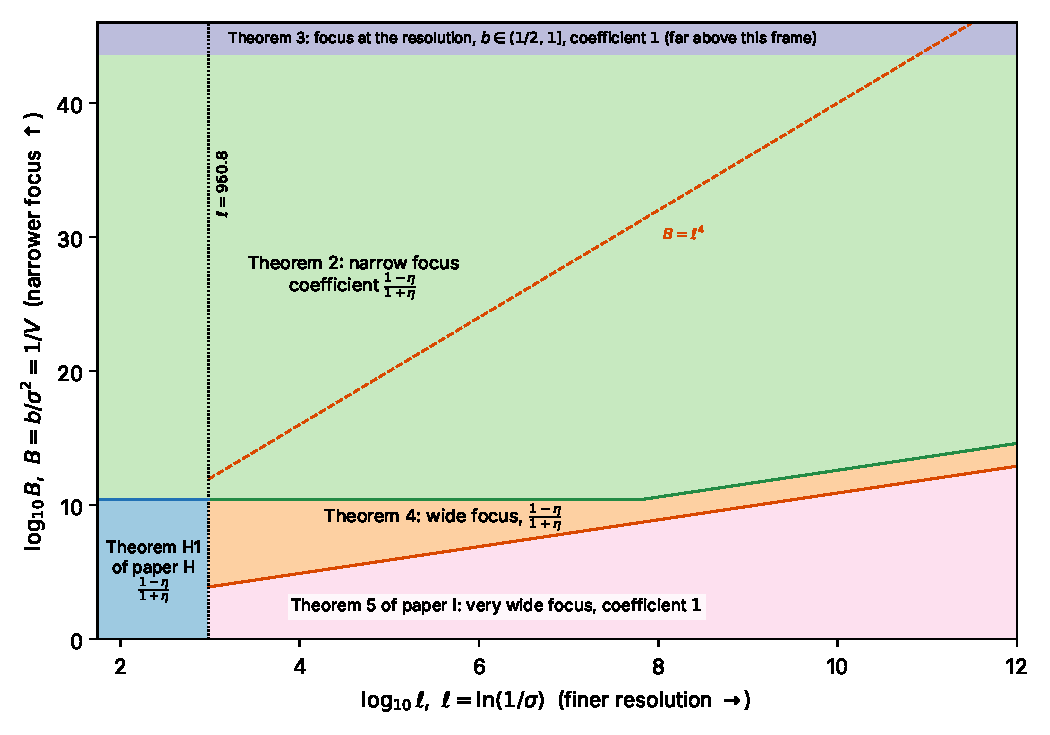
\includegraphics[width=\columnwidth]{figures/fig_map_J.pdf}
\caption{The map of the states in the $(\ell,B)$ plane, $B=b/\sigma^2$, with the coefficient that each room proves for every admissible window: $(1-\eta)/(1+\eta)=\lambda/\Upsilon$ in the narrow and wide rooms and in Theorem~H1 of~\cite{H}, one at the resolution and in the very wide room. The boundaries are those of Paper~I~\cite{I}.}
\label{fig:map}
\end{figure}

\subsection{Proof of Theorem~\ref{thm:J} from the rooms}
\begin{proof}
The case split is that of Theorem~1 of~\cite{I} (Sec.~II~C there), word for word, with the four rooms of Table~\ref{tab:rooms} in place of those of~\cite{I}.
Each room gives $(a)+(a')\ge c\,\Gamma_\ell$ with $c\in\{1,\lambda/\Upsilon\}$, so $c\ge\lambda/\Upsilon$; Theorem~H1 gives the bound on $g\sqrt\ell$ directly, with $1+12.1/\ell+2.5\times10^{-4}\ge1$.
Eq.~\eqref{eq:ga} and $\Gamma_\ell\sqrt\ell=\sqrt{1+10/\ell}$ give both statements.
\end{proof}

\subsection{What is borrowed and what is new}
\begin{itemize}
\item Borrowed unchanged: Eq.~\eqref{eq:ga} and the class conditions~\cite{F}; Theorem~H1, Lemma~CM-1, Lemma~R$_\theta$ and the sandwich~\cite{H}; the local lemmas, the 37 lines with $\eta$ as a parameter, the brightness lemma (H$'$), Lemma~$G=0$, the rule of the proof and Theorem~5~\cite{I}.
\item New here: the chord lemma (Lemma~\ref{lem:chord}) and the scaled target (Sec.~\ref{sec:sandwich}); the repaired step of FrB1 (Sec.~\ref{sec:changes}); the constants of the rule, the 18 new quoted bounds, the allocation of the remainder budget and the tail (Sec.~\ref{sec:changes}, Apps.~\ref{app:B}--\ref{app:C}); the interval proofs at the two ends (App.~\ref{app:D}); the hand proof of Theorem~\ref{thm:Jres} for every ripple (Sec.~\ref{sec:res}).
\end{itemize}
